% /**
%  * A template for homework files in math classes. The 
%  * packages and newcommands are a good starting point.
%  *
%  * Author: James K. Pringle
%  * E-mail: jameskpringle@gmail.com
%  * Last Changed: 5 September 2013
%  *
%  * "LaTeX countains the increasing union of MS Word"
%  */
%~~~~~~~~~~~~~~~~~~~~~~~~~~~~~~~~~~~~~~~~~~~~~~~~~~~~~~~~~%
%%%%%%%%%%%%%%%%%%%%%%%%%%%%%%%%%%%%%%%%%%%%%%%%%%%%%%%%%%%
%                                                         %
%                        PAGE SETUP                       %
%                                                         %
%%%%%%%%%%%%%%%%%%%%%%%%%%%%%%%%%%%%%%%%%%%%%%%%%%%%%%%%%%%
\documentclass[letterpaper, 12pt]{article}\usepackage[]{graphicx}\usepackage[]{color}
%% maxwidth is the original width if it is less than linewidth
%% otherwise use linewidth (to make sure the graphics do not exceed the margin)
\makeatletter
\def\maxwidth{ %
  \ifdim\Gin@nat@width>\linewidth
    \linewidth
  \else
    \Gin@nat@width
  \fi
}
\makeatother

\definecolor{fgcolor}{rgb}{0.345, 0.345, 0.345}
\newcommand{\hlnum}[1]{\textcolor[rgb]{0.686,0.059,0.569}{#1}}%
\newcommand{\hlstr}[1]{\textcolor[rgb]{0.192,0.494,0.8}{#1}}%
\newcommand{\hlcom}[1]{\textcolor[rgb]{0.678,0.584,0.686}{\textit{#1}}}%
\newcommand{\hlopt}[1]{\textcolor[rgb]{0,0,0}{#1}}%
\newcommand{\hlstd}[1]{\textcolor[rgb]{0.345,0.345,0.345}{#1}}%
\newcommand{\hlkwa}[1]{\textcolor[rgb]{0.161,0.373,0.58}{\textbf{#1}}}%
\newcommand{\hlkwb}[1]{\textcolor[rgb]{0.69,0.353,0.396}{#1}}%
\newcommand{\hlkwc}[1]{\textcolor[rgb]{0.333,0.667,0.333}{#1}}%
\newcommand{\hlkwd}[1]{\textcolor[rgb]{0.737,0.353,0.396}{\textbf{#1}}}%

\usepackage{framed}
\makeatletter
\newenvironment{kframe}{%
 \def\at@end@of@kframe{}%
 \ifinner\ifhmode%
  \def\at@end@of@kframe{\end{minipage}}%
  \begin{minipage}{\columnwidth}%
 \fi\fi%
 \def\FrameCommand##1{\hskip\@totalleftmargin \hskip-\fboxsep
 \colorbox{shadecolor}{##1}\hskip-\fboxsep
     % There is no \\@totalrightmargin, so:
     \hskip-\linewidth \hskip-\@totalleftmargin \hskip\columnwidth}%
 \MakeFramed {\advance\hsize-\width
   \@totalleftmargin\z@ \linewidth\hsize
   \@setminipage}}%
 {\par\unskip\endMakeFramed%
 \at@end@of@kframe}
\makeatother

\definecolor{shadecolor}{rgb}{.97, .97, .97}
\definecolor{messagecolor}{rgb}{0, 0, 0}
\definecolor{warningcolor}{rgb}{1, 0, 1}
\definecolor{errorcolor}{rgb}{1, 0, 0}
\newenvironment{knitrout}{}{} % an empty environment to be redefined in TeX

\usepackage{alltt}

% 1in margins all the way around
\usepackage[margin=1in]{geometry}

% Sets \parindent to 0 and \parskip to stretchable.
\usepackage{parskip}
% Use for bigger spaces between paragraphs.
%\parskip=1.5\baselineskip

% Set headers and footers
\usepackage{fancyhdr}
\pagestyle{fancy}
% Header
\renewcommand{\headrulewidth}{0.4pt}
\lhead{\textsc{\mathclass}}
\chead{\textsc{\today}}
\rhead{\textsc{\mynamehdr}}
% Footer
\renewcommand{\footrulewidth}{0.4pt}
\lfoot{}
\cfoot{\thepage}
\rfoot{}

% Make the space between lines slightly more generous 
% than normal single spacing, but compensate so that the 
% spacing between rows of matrices still looks normal.  
% Note that 1.1=1/.9090909...
\renewcommand{\baselinestretch}{1.1}
\renewcommand{\arraystretch}{.91}

%%%%%%%%%%%%%%%%%%%%%%%%%%%%%%%%%%%%%%%%%%%%%%%%%%%%%%%%%%%
%                                                         %
%                      USEFUL PACKAGES                    %
%                                                         %
%%%%%%%%%%%%%%%%%%%%%%%%%%%%%%%%%%%%%%%%%%%%%%%%%%%%%%%%%%%

% The classic three
\usepackage{amsmath,amsthm,amssymb}

% Define \newtheorem for use
% No numbers, labeled 'Theorem'
\newtheorem*{nthm}{Theorem}

% Not sure what this is for
\usepackage{amsfonts}

% Fancy script font
\usepackage{mathrsfs}

% Makes enumerate environment much easier to customize
% by specifying the counter
\usepackage{enumerate}

% Color
\usepackage{color}
\usepackage[usenames,dvipsnames,svgnames,table]{xcolor}

% URL links
\usepackage{hyperref}

% For inserting graphics and images
\usepackage{graphicx}
\usepackage{float}
\usepackage[footnotesize]{caption}



%%%%%%%%%%%%%%%%%%%%%%%%%%%%%%%%%%%%%%%%%%%%%%%%%%%%%%%%%%%
%                                                         %
%                   USER-DEFINED COMMANDS                 %
%                                                         %
%%%%%%%%%%%%%%%%%%%%%%%%%%%%%%%%%%%%%%%%%%%%%%%%%%%%%%%%%%%

% Make a hyperlink with colored text
\newcommand{\hrefcolor}[3]{\href{#1}{\textcolor{#3}{#2}}}

% Make a hyperlink with gray text
\newcommand{\hrefgray}[2]{\hrefcolor{#1}{#2}{Gray}}

% Make the header for the first page
\newcommand{\firstpageinfo}{
\textsf{
\begin{flushleft}
\sc \myname \\
\normalfont \mathclass \\
\professorname \\
\assignmentnumber \\
\thedate
\end{flushleft}
} \bigskip
}

% Make problem list for "title" of page
\newcommand{\problemlist}{ 
\begin{center}
\textbf{\Large \textsf{\assignmentnumber}}\\
\textit{\textsf{\problemset}}
\end{center}
\bigskip
}

%~~~~~~~~~~~~~~~~~~~~~~~~~~~~~~~~~~~~~~~~~~~~~~~~~~~~~~~~~%
%                                                         %
%               LETTERS, FUNCTIONS, AND TEXT              %
%                                                         %
%~~~~~~~~~~~~~~~~~~~~~~~~~~~~~~~~~~~~~~~~~~~~~~~~~~~~~~~~~%

% A
\newcommand{\cA}{\mathcal{A}}
\newcommand{\sA}{\mathscr{A}}
\renewcommand{\aa}{\;\text{a.a.}}
\renewcommand{\ae}{\;\text{a.e.}}
% B
\newcommand{\B}{\mathscr{B}}
\newcommand{\cB}{\mathcal{B}}
% C
\newcommand{\cC}{\mathcal{C}}
\newcommand{\cov}{\text{cov}}
% E
\newcommand{\E}{\mathbb{E}}
% F
\newcommand{\sF}{\mathscr{F}}
\newcommand{\cF}{\mathcal{F}}
\newcommand{\Ft}{F^\sim}
% G
\newcommand{\cG}{\mathcal{G}}
\newcommand{\sG}{\mathscr{G}}
% H
\newcommand{\bh}{\mathbf{h}}
% I
\newcommand{\io}{\;\text{i.o.}}
% N
\newcommand{\N}{\mathbb{N}}
% P
\newcommand{\cP}{\mathcal{P}}
\newcommand{\sP}{\mathscr{P}}
\newcommand{\pr}{\text{pr}}
% Q
\newcommand{\Q}{\mathbb{Q}}
% R
\newcommand{\R}{\mathbb{R}}
\newcommand{\bR}{\mathbf{R}}
\newcommand{\cR}{\mathcal{R}}
% S
\newcommand{\cS}{\mathcal{S}}
% U
\newcommand{\cU}{\mathcal{U}}
% V
\newcommand{\var}{\text{var}}
% Z
\newcommand{\Z}{\mathbb{Z}}
% Punctuation
\newcommand{\sbs}{\;|\;} % space bar space
% Math
\newcommand{\imii}{\int_{-\infty}^\infty}
\newcommand{\pion}{\prod_{i=1}^n}
\newcommand{\pioI}{\prod_{i=1}^I}
\newcommand{\pjon}{\prod_{j=1}^n}
\newcommand{\pjoJ}{\prod_{j=1}^J}
\newcommand{\pkon}{\prod_{k=1}^n}
\newcommand{\pkoK}{\prod_{k=1}^K}
\newcommand{\sion}{\sum_{i=1}^n}
\newcommand{\sioI}{\sum_{i=1}^I}
\newcommand{\sjon}{\sum_{j=1}^n}
\newcommand{\sjoJ}{\sum_{j=1}^J}
\newcommand{\skon}{\sum_{k=1}^n}
\newcommand{\skoK}{\sum_{k=1}^K}
\newcommand{\sioi}{\sum_{i=1}^\infty}
\newcommand{\sjoi}{\sum_{j=1}^\infty}
\newcommand{\skoi}{\sum_{k=1}^\infty}
\newcommand{\sio}{\sum_{i=1}}
\newcommand{\sjo}{\sum_{j=1}}
\newcommand{\sko}{\sum_{k=1}}
% Typography
\newcommand{\scb}[1]{\textsc{\textbf{#1}}}

%~~~~~~~~~~~~~~~~~~~~~~~~~~~~~~~~~~~~~~~~~~~~~~~~~~~~~~~~~%
%                                                         %
%            CHANGE THESE BASED ON THE PAPER              %
%                                                         %
%~~~~~~~~~~~~~~~~~~~~~~~~~~~~~~~~~~~~~~~~~~~~~~~~~~~~~~~~~%

% Constants for fancy header and first page info
\newcommand{\mynamehdr}{\hrefgray{http://biostat.jhsph.edu/~jpringle/}{\myname}}
\newcommand{\mathclass}{140.663 Geostatistics}
\newcommand{\myname}{James K. Pringle}
\newcommand{\professorname}{Dr. Curriero}
\newcommand{\assignmentnumber}{Assignment 3}
\newcommand{\thedate}{\today}
\newcommand{\problemset}{Questions 5}

%%%%%%%%%%%%%%%%%%%%%%%%%%%%%%%%%%%%%%%%%%%%%%%%%%%%%%%%%%%
%                                                         %
%                      BEGIN DOCUMENT                     %
%                                                         %
%%%%%%%%%%%%%%%%%%%%%%%%%%%%%%%%%%%%%%%%%%%%%%%%%%%%%%%%%%%
\IfFileExists{upquote.sty}{\usepackage{upquote}}{}
\begin{document}

% Take header off of first page
\thispagestyle{empty}

% Put in first page info (top of page)
\firstpageinfo

% Put in title for the paper
\problemlist

%%%%%%%%%%%%%%%%%%%%%%%%%%%%%%%%%%%%%%%%%%%%%%%%%%%%%%%%%%%
%                                                         %
%                     Start Problem 1                     %
%                                                         %
%%%%%%%%%%%%%%%%%%%%%%%%%%%%%%%%%%%%%%%%%%%%%%%%%%%%%%%%%%%
\setcounter{section}{4}
\section{Kriging the EPA’s AQS Ozone Data.}
This data set corresponds to the EPA’s AQS average annual daily 8 hour maximum ozone for 2007. The questions and code provided run through a kriging analysis of this data based on several different approaches. 
All the data you will need for this problem are in the two zipped folders 
\texttt{Ozone\_Monitors\_2007\_reproj} 
and 
\texttt{States\_reproj\_lower48} 
posted on Courseplus. Unzip these and save them in your R working directory.

\subsection*{Exploratory Spatial Data Analysis of the Ozone Data}
\begin{enumerate}[a.]
\item
Produce a map of ozone with symbols signifying magnitude.




\begin{knitrout}
\definecolor{shadecolor}{rgb}{0.969, 0.969, 0.969}\color{fgcolor}
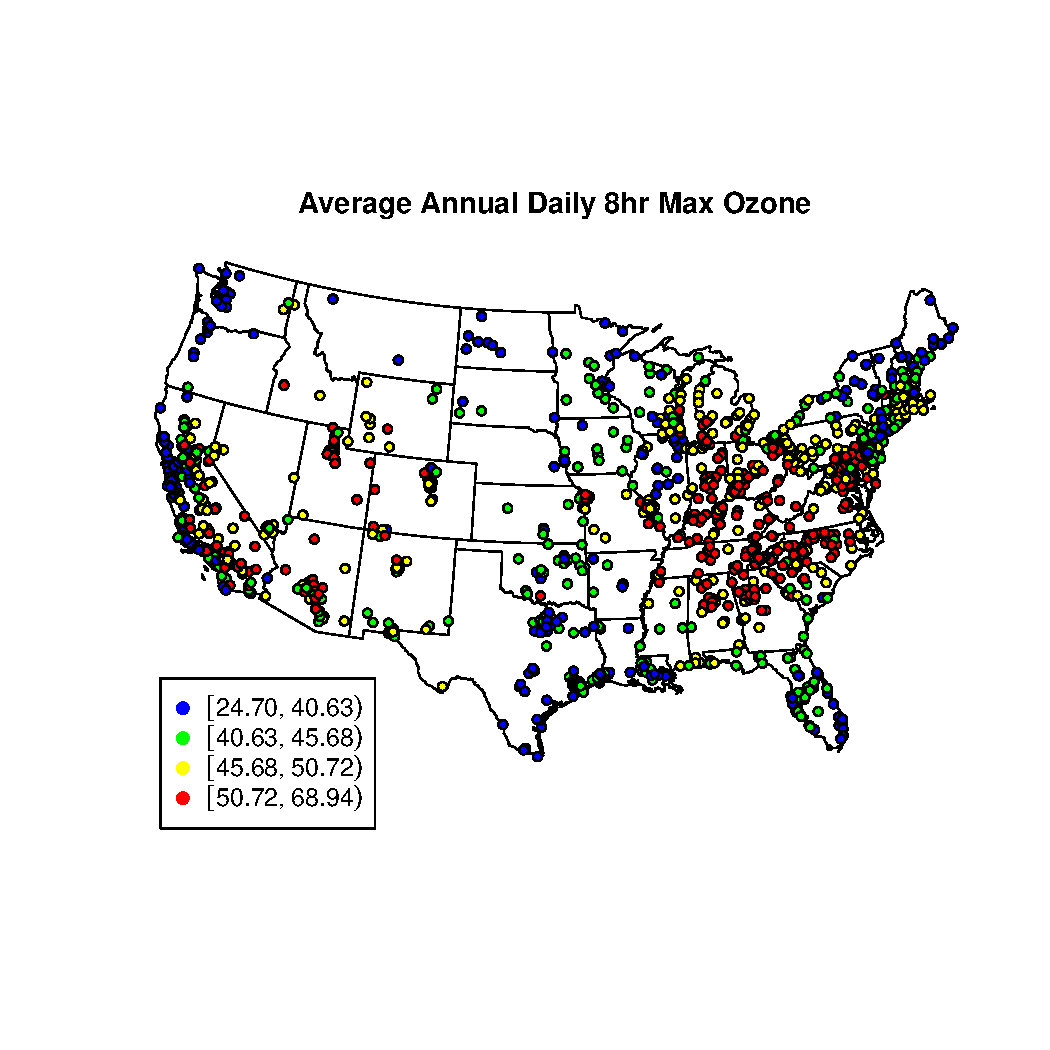
\includegraphics[width=\maxwidth]{figure/ozonemap} 

\end{knitrout}


\item
Produce a $2\times 2$ display of 4 descriptive plots using the \texttt{plot(geodata object)} command for the ozone data. This is a large area to consider, so to better see possible spatial trends across the US, plot the data separately versus the $x$ and $y$ coordinates.

\begin{knitrout}
\definecolor{shadecolor}{rgb}{0.969, 0.969, 0.969}\color{fgcolor}
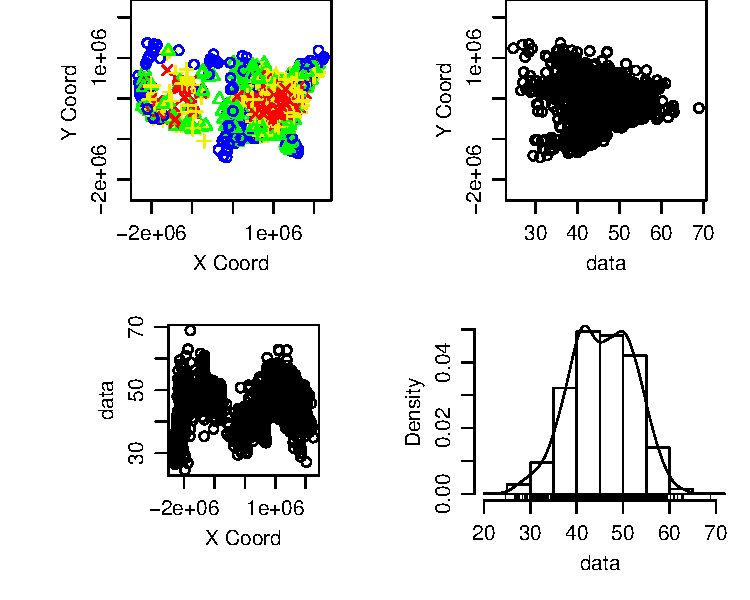
\includegraphics[width=\maxwidth]{figure/twoxtwo} 

\end{knitrout}


\begin{knitrout}
\definecolor{shadecolor}{rgb}{0.969, 0.969, 0.969}\color{fgcolor}
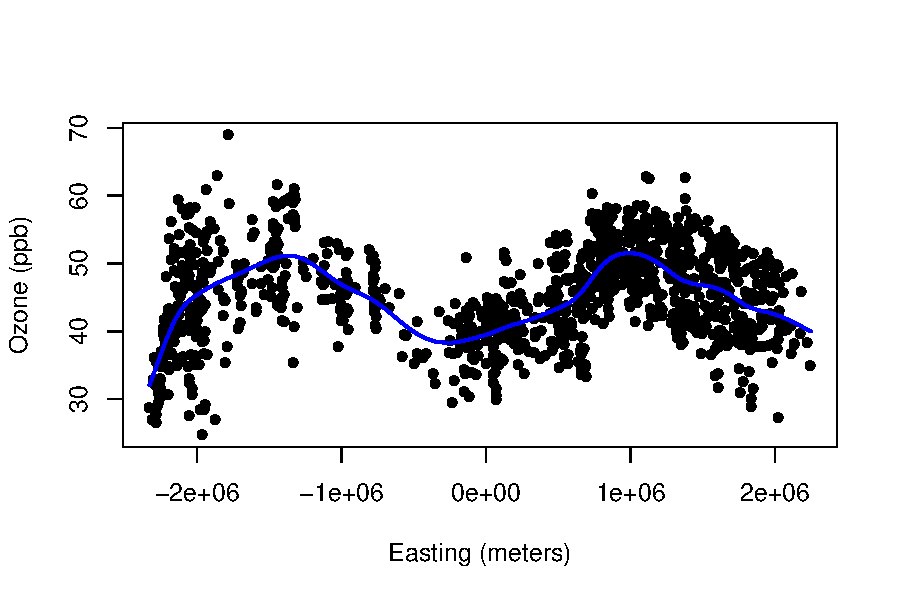
\includegraphics[width=\maxwidth]{figure/xcoord} 

\end{knitrout}


\begin{knitrout}
\definecolor{shadecolor}{rgb}{0.969, 0.969, 0.969}\color{fgcolor}
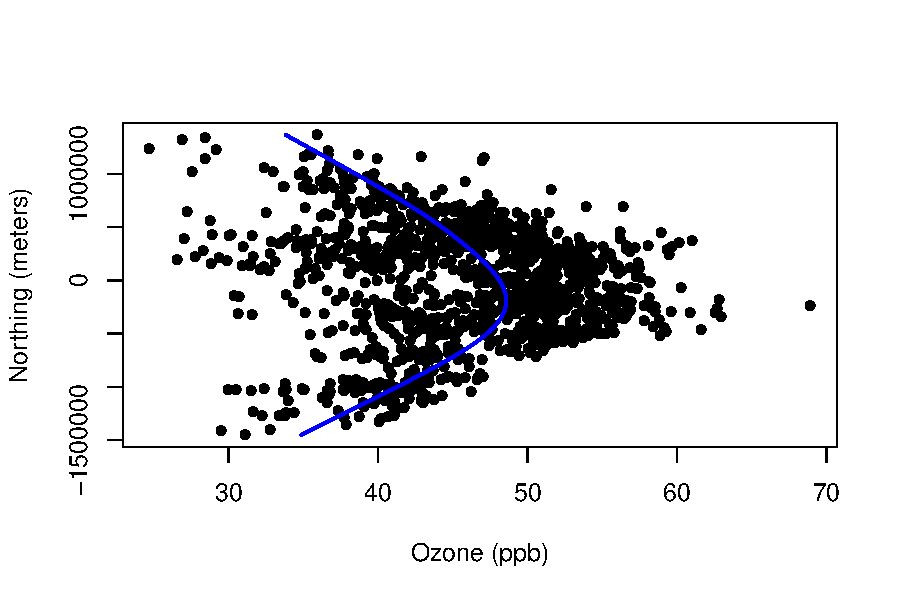
\includegraphics[width=\maxwidth]{figure/ycoord} 

\end{knitrout}


\item
Estimate and plot the semivariogram of the ozone data using the default binning in \texttt{variog}.
Actually estimate and plot the semivariogram with and without restricting the distances to be within half the maximum inter-point distance (so estimate two semivariograms). In the future though whenever asked to estimate a semivariogram/variogram always restrict it to be within half the maximum inter-point distance.

\begin{knitrout}
\definecolor{shadecolor}{rgb}{0.969, 0.969, 0.969}\color{fgcolor}
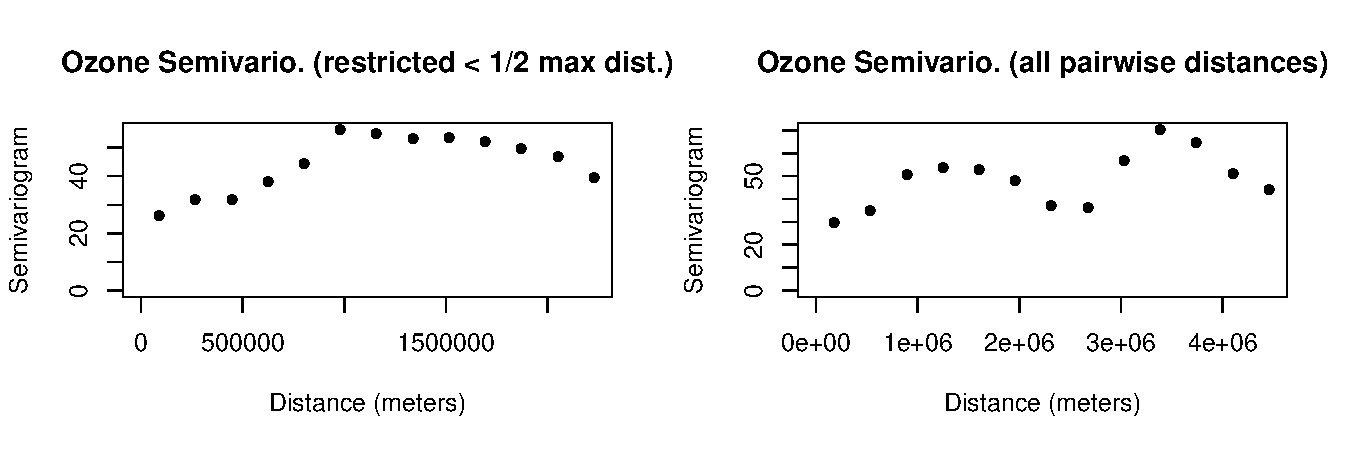
\includegraphics[width=\maxwidth]{figure/vario} 

\end{knitrout}


\item
For the ozone semivariogram based on distances restricted to be within half the maximum inter-point distance use the \texttt{eyefit} command and select a semivariogram function and set of parameter estimates that appear to fit the semivariogram well. For Mac users who have problem getting the \texttt{eyefit} command to work just eyeball a set of parameter estimates.

\begin{knitrout}
\definecolor{shadecolor}{rgb}{0.969, 0.969, 0.969}\color{fgcolor}
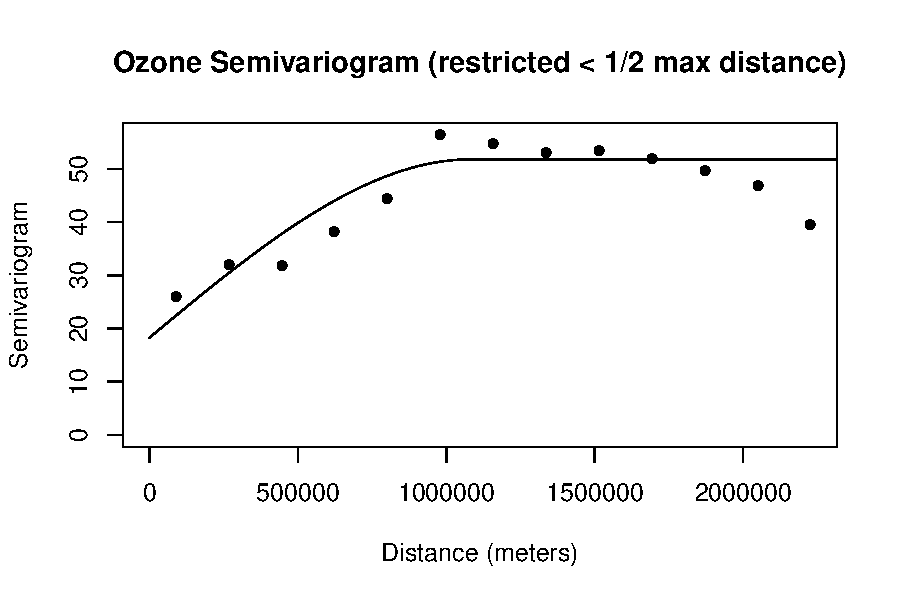
\includegraphics[width=\maxwidth]{figure/variofit} 

\end{knitrout}


\textsf{This is a spherical variogram function with parameters}
\begin{itemize}
\item
$\phi = \ensuremath{1.0833\times 10^{6}}$
\item
$\tau^2 = 18.28$
\item
$\sigma^2 = 33.51$
\end{itemize}

\item
Following the results from (b) go ahead a fit a large scale spatial trend based on the easting (or $x$) coordinate, ignoring and trend in the northing (or $y$) coordinate. 
The code I provide fits a natural spline of the easting coordinate with 4 degrees of freedom to try and match the apparent trend. 
Now using the residuals from this model, estimate and plot the semivariogram (residual semivariogram) and use the \texttt{eyefit} command and select a semivariogram function and set of parameter estimates that appear to fit the semivariogram well. Select the same semivariogram function as you did in (d).

\begin{knitrout}
\definecolor{shadecolor}{rgb}{0.969, 0.969, 0.969}\color{fgcolor}
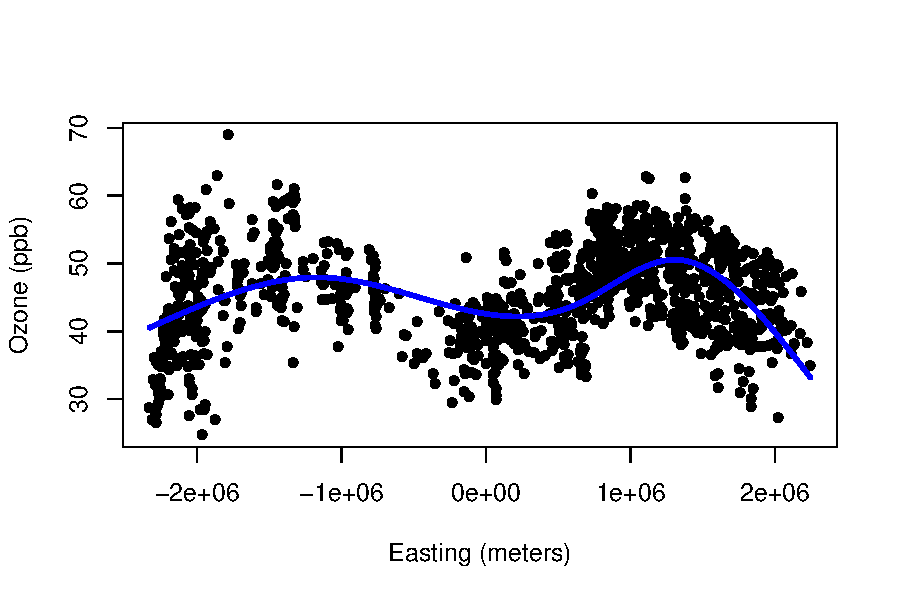
\includegraphics[width=\maxwidth]{figure/natspline} 

\end{knitrout}


\begin{knitrout}
\definecolor{shadecolor}{rgb}{0.969, 0.969, 0.969}\color{fgcolor}
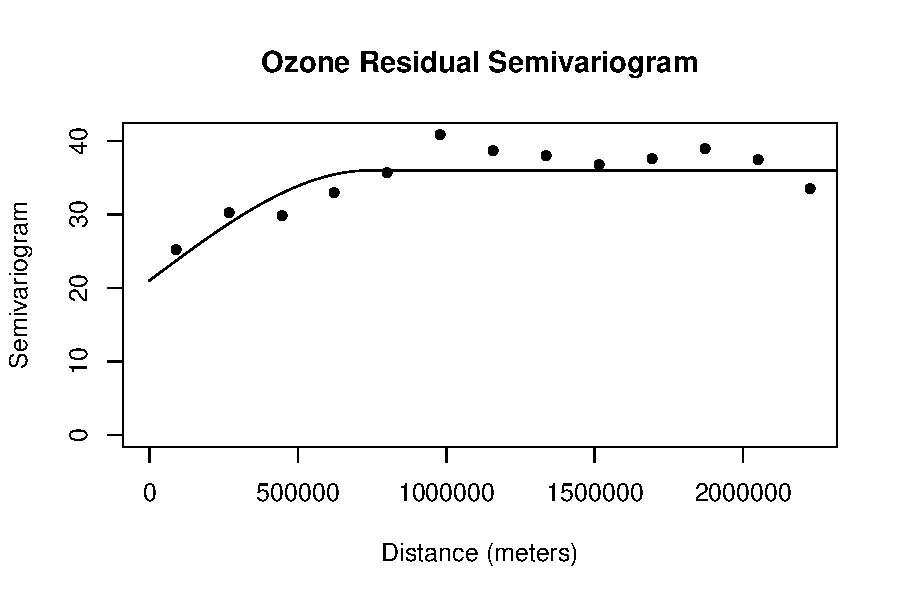
\includegraphics[width=\maxwidth]{figure/residfit} 

\end{knitrout}


\textsf{This is a spherical semivariogram function with parameters}
\begin{itemize}
\item
$\phi = \ensuremath{7.4228\times 10^{5}}$
\item
$\tau^2 = 21$
\item
$\sigma^2 = 15$
\end{itemize}

\item
With the information generated (a) - (e) address the following and reference specific plots in your answers/interpretations.
\begin{enumerate}[(i)]
\item
Does the ozone data appear to be Normally distributed?

{\sf
The data do appear to be Normally distributed according to the density and histogram from the $2 \times 2$ plot above in part b.
}
\item
Argue for the existence of a large scale spatial trend in the ozone data.

{\sf
We have examined the relationship between the easting and northing coordinates and the outcome (ozone). Both the easting and the northing component seem to have a nonlinear relationship with ozone, as can be seen in the plots under part b. If there were no relationship, we would expect the scatter plots in b. to be more of a uniform blob of points. In contrast, the scatter plots in b. seem to have a pattern. Therefore, knowing the value of the easting and the northing coordinates gives at least some knowledge of the ozone amount.
}
\item
Describe the difference in the two estimated semivariograms from (c) and what might be influencing the pattern seen in the semivariogram estimated based on all pairwise distances.

{\sf
Obviously, the semivariogram which has distances up to the maximum distance contains the semivariogram restricted to half the distance. However, in the full semivariogram, the data has bigger bins than in the restricted semivariogram. The full semivariogram shows that beyond half the max distance, the variance dips (around 2.5 Mm, where Mm means megameter) then spikes (around 3.5 Mm) then settles down again (around 4.5 Mm) as the distance decreases. 

It seems from the plot of Ozone vs. Easting that the two peaks in the spline are about 2.5 Mm apart. Since the fitted trend seems sinusoidal, with period about 2.5 Mm, then it would be reasonable that points that far apart would show a lower variance (values are more similar than different as shown by the spline). Furthermore, 2.5 Mm is about the maximum difference  in the northing coordinates, so the points that are 2.5 Mm apart and more are separated more along an East-West line than a North-South line. The spike at 3.5 Mm might be related to the fitted trend (it is about there that we have a period and a half in the Ozone vs. Easting trend).  
}
\item
Specify the spatial regression model (its either ordinary or universal kriging) for what the semivariogram estimated in (c) is for and what the semivariogram estimated in (e) is for. 
So two models need to be specified. 
Also for each describe what data the semivariogram is estimating spatial dependence of.

{\sf
In (c) the model is ordinary kriging. It is 
\[
Y(s) = b_0 + \epsilon(s)
\]
and here $\epsilon(s) \sim N(0, \Sigma)$. The variance matrix $\Sigma$ is estimated with the spherical model to approximate the semivariogram. The parameters for the spherical model are
\begin{itemize}
\item
$\phi = \ensuremath{1.0833\times 10^{6}}$
\item
$\tau^2 = 18.28$
\item
$\sigma^2 = 33.51$
\end{itemize}
Here the semivariogram estimates the spatial dependence of the data $Y(s)$, the geotagged ozone quantities. 

In (e) the model is universal kriging,
\[
Y(s) = b_0 + b_1 X(s) + \epsilon(s)
\]
Here, $X(s)$ represents the value of the natural spline estimated from Ozone vs. Easting. Thus $X(s)$ is only a function of the easting coordinate. The error structure is 
\[
\epsilon \sim N(0, \Sigma)
\]
where the variance matrix $\Sigma$ is estimated with the spherical model to apprximate the semivariogram. The parameters for this spherical model are
\begin{itemize}
\item
$\phi = \ensuremath{7.4228\times 10^{5}}$
\item
$\tau^2 = 21$
\item
$\sigma^2 = 15$
\end{itemize}
Here the semivariogram estimates the spatial dependence of the residuals of $Y(s)$, the ozone data, after accounting for the value of the natural spline at $s$.
}
\item
Describe any difference in the fitted semivariogram functions arrived at in (d) and (e). 
How have the total sills changed and provide an interpretation for this?

{\sf
The total sill is different in the fitted semivariograms. The covariate (the natural spline value at the easting coordinate) accounted for some of the spatial variation in the outcome (ozone). Therefore the residuals have less spatial variation (less total sill) than the outcome data do. That is why the fitted semivariogram for the residuals levels off at a lower value than the fitted semivariogram for the outcome data.
}
\end{enumerate}
\end{enumerate}

\subsection*{Kriging the ozone data}
\begin{enumerate}
\item[g.]
Using weighted least squares, fit the semivariogram function from (d) to the ozone data using the initial values selected in (d). Again using weighted least squares fit the semivariogram function from (e) to the residuals of the model used in (e) using the initial values selected.

\begin{knitrout}
\definecolor{shadecolor}{rgb}{0.969, 0.969, 0.969}\color{fgcolor}
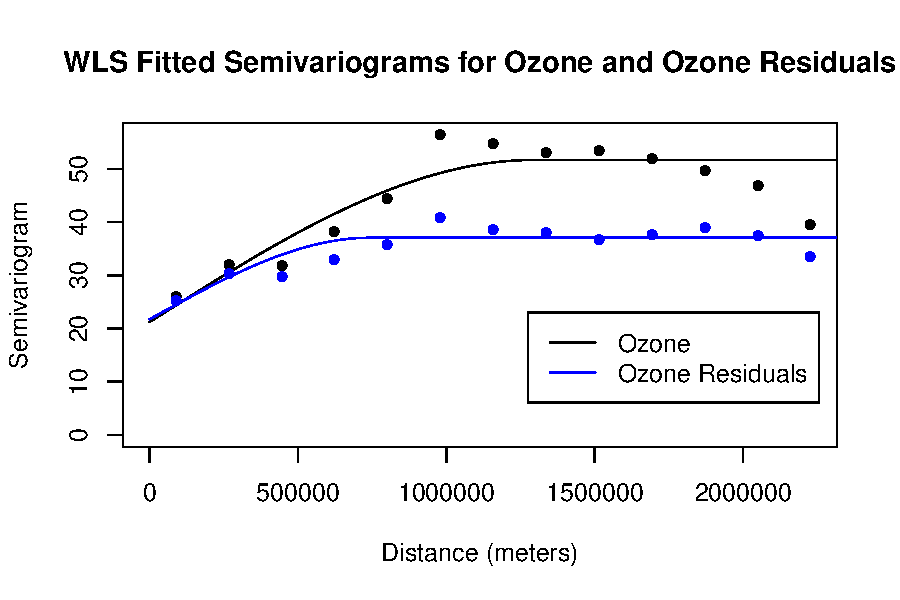
\includegraphics[width=\maxwidth]{figure/krig} 

\end{knitrout}


\item[h.]
Produce a map of IDW predicted ozone.

\begin{knitrout}
\definecolor{shadecolor}{rgb}{0.969, 0.969, 0.969}\color{fgcolor}
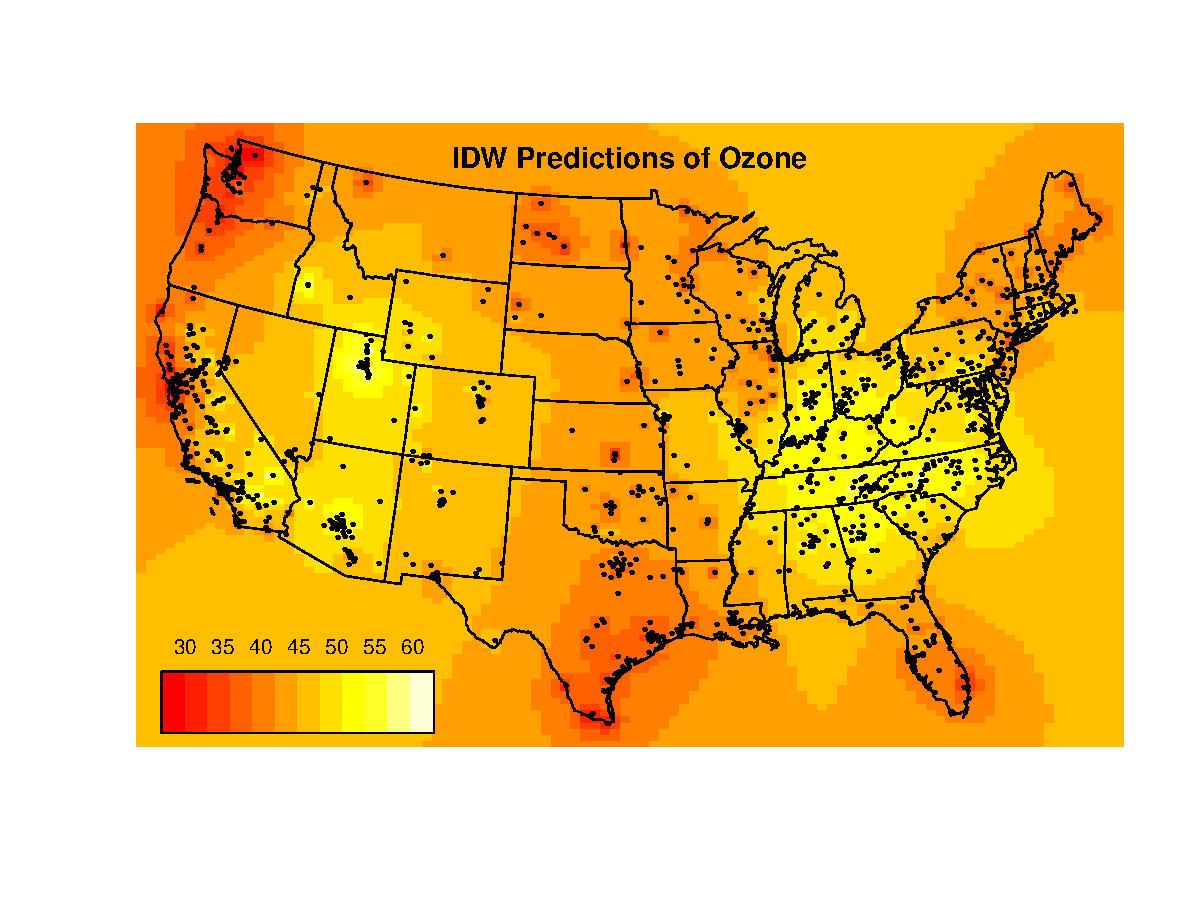
\includegraphics[width=\maxwidth]{figure/idw} 

\end{knitrout}


\item[i.]
Produce a map of trend surface model ozone predictions and a map of predicted stan- dard errors. Specify the trend using the natural spline (with 4 degrees of freedom) of the easting coordinate as utilized previously.

\begin{knitrout}
\definecolor{shadecolor}{rgb}{0.969, 0.969, 0.969}\color{fgcolor}
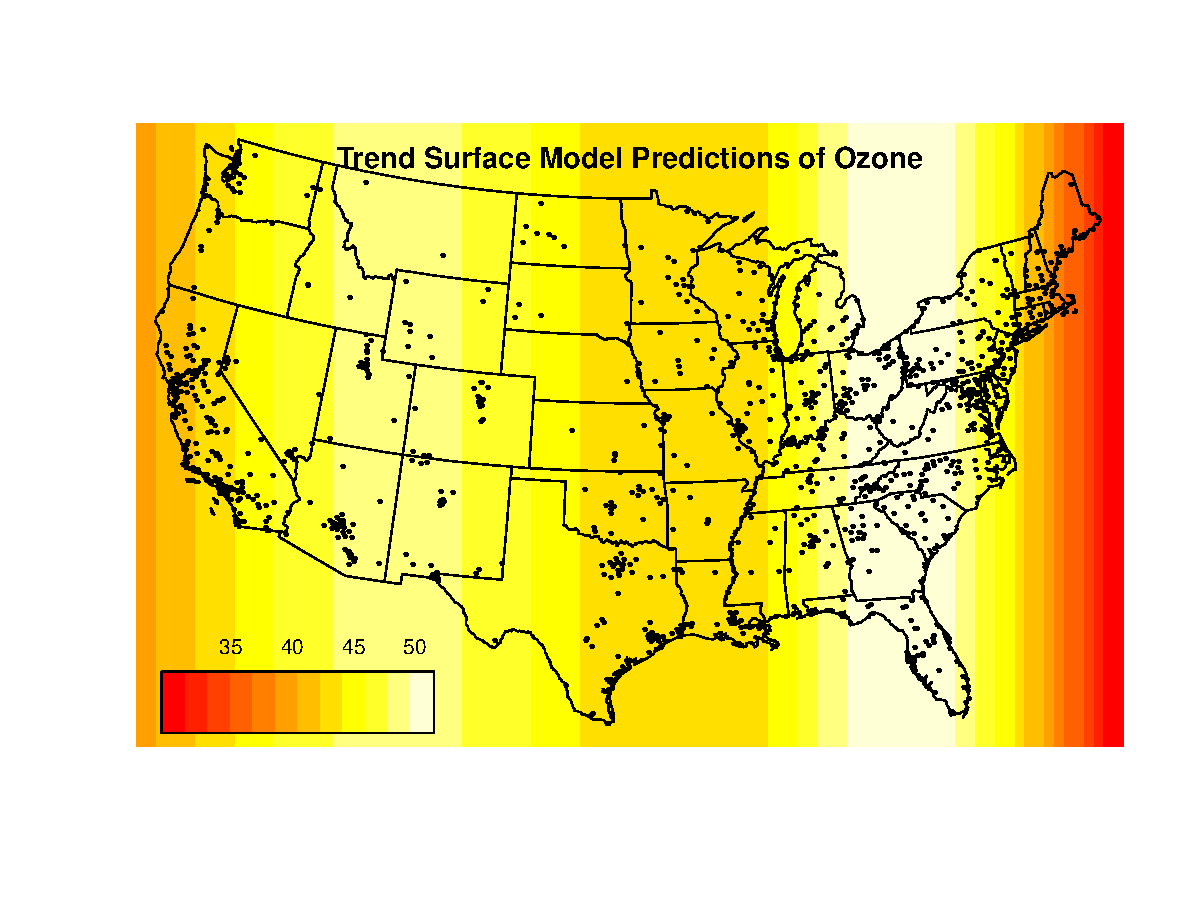
\includegraphics[width=\maxwidth]{figure/ts} 

\end{knitrout}


\begin{knitrout}
\definecolor{shadecolor}{rgb}{0.969, 0.969, 0.969}\color{fgcolor}
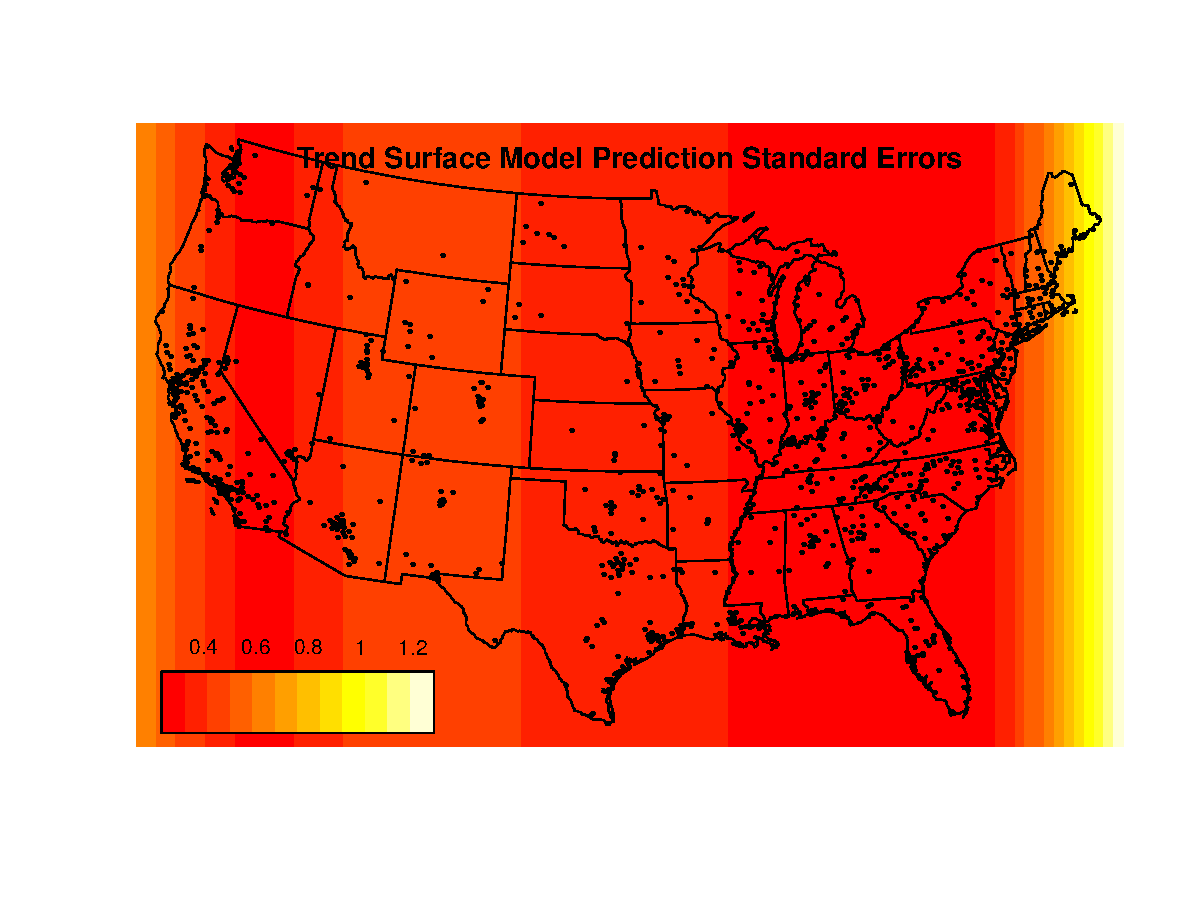
\includegraphics[width=\maxwidth]{figure/tsresid} 

\end{knitrout}

\item[j.]
Produce a map of ordinary kriged ozone predictions and a map of corresponding prediction standard errors.

\begin{knitrout}
\definecolor{shadecolor}{rgb}{0.969, 0.969, 0.969}\color{fgcolor}
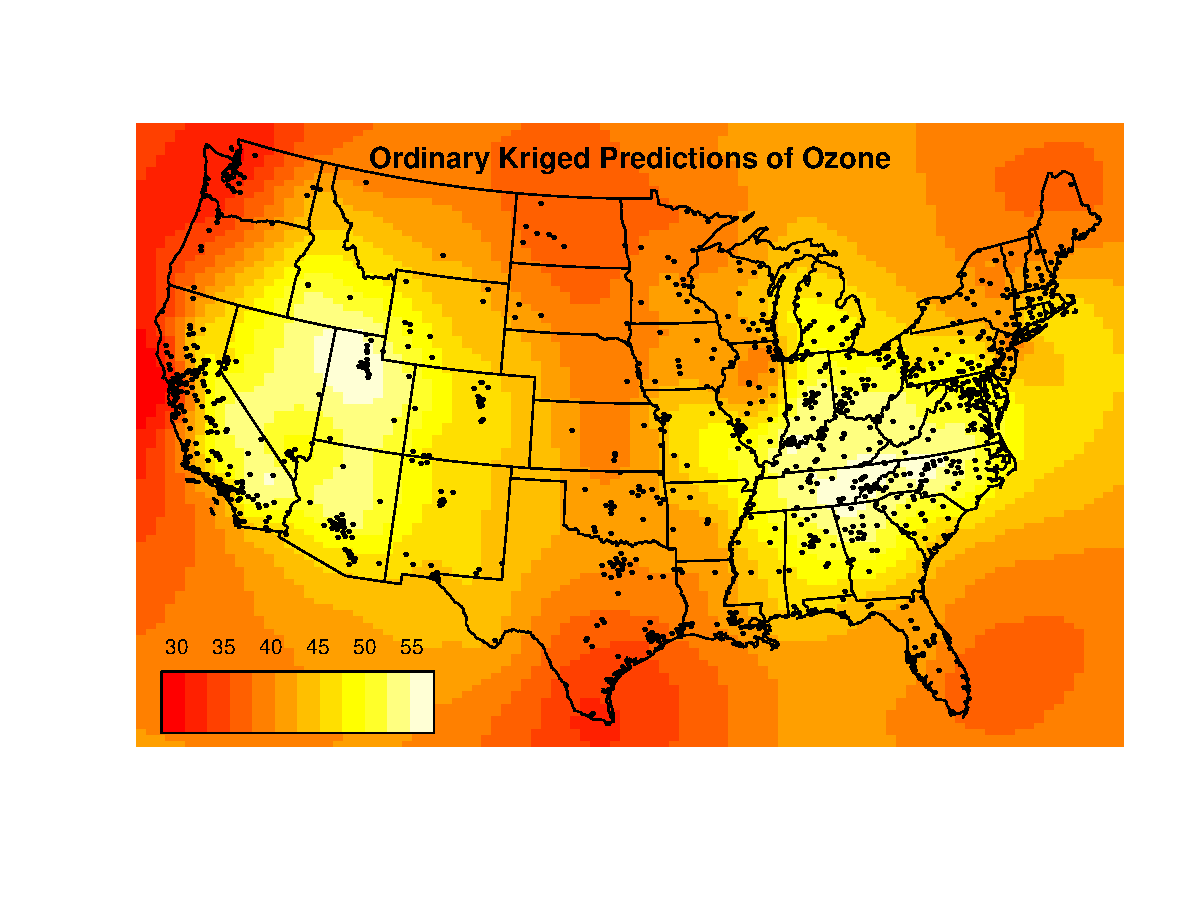
\includegraphics[width=\maxwidth]{figure/ok} 

\end{knitrout}


\begin{knitrout}
\definecolor{shadecolor}{rgb}{0.969, 0.969, 0.969}\color{fgcolor}
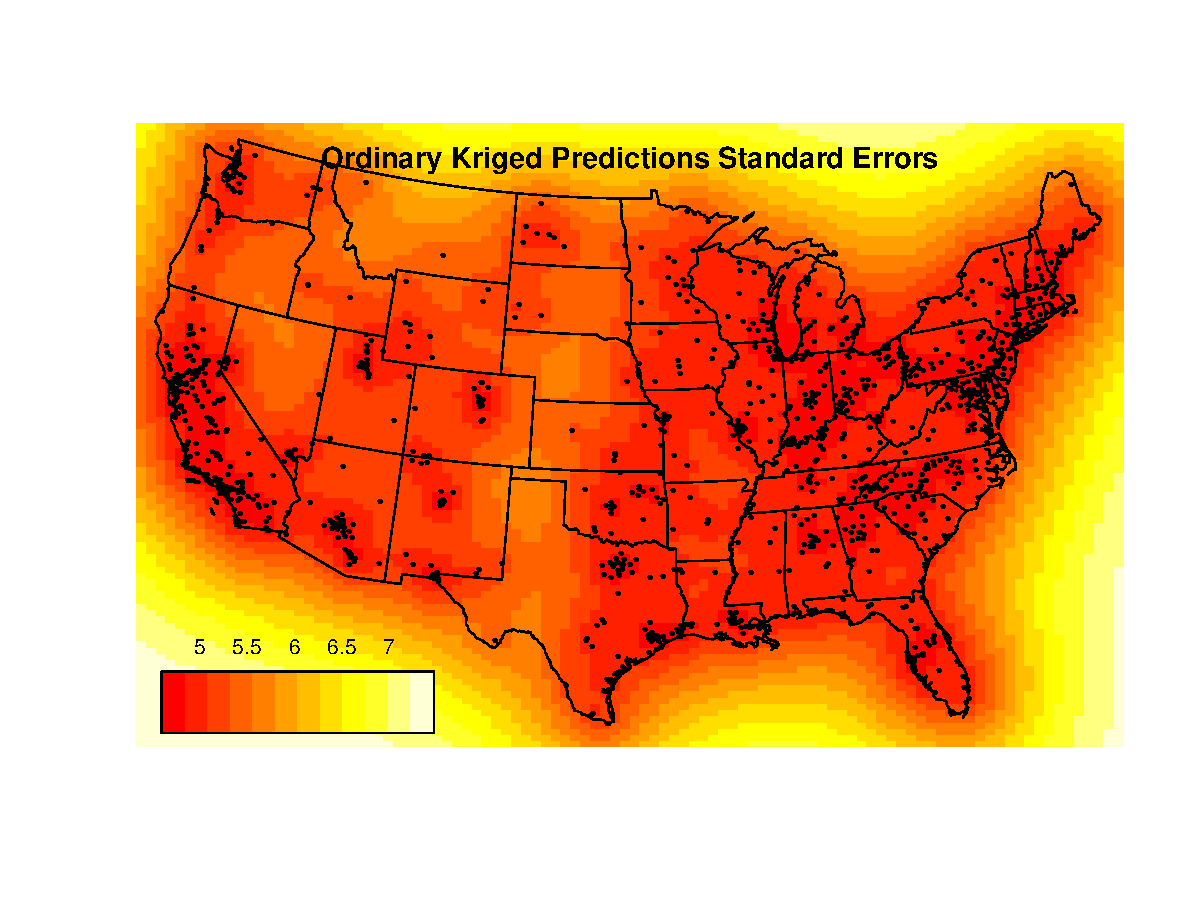
\includegraphics[width=\maxwidth]{figure/okresid} 

\end{knitrout}


\item[k.]
Produce a map of universal kriged ozone predictions and a map of corresponding prediction standard errors. For the trend use the same natural spline on the easting coordinate as in the trend surface model predictions.

\begin{knitrout}
\definecolor{shadecolor}{rgb}{0.969, 0.969, 0.969}\color{fgcolor}
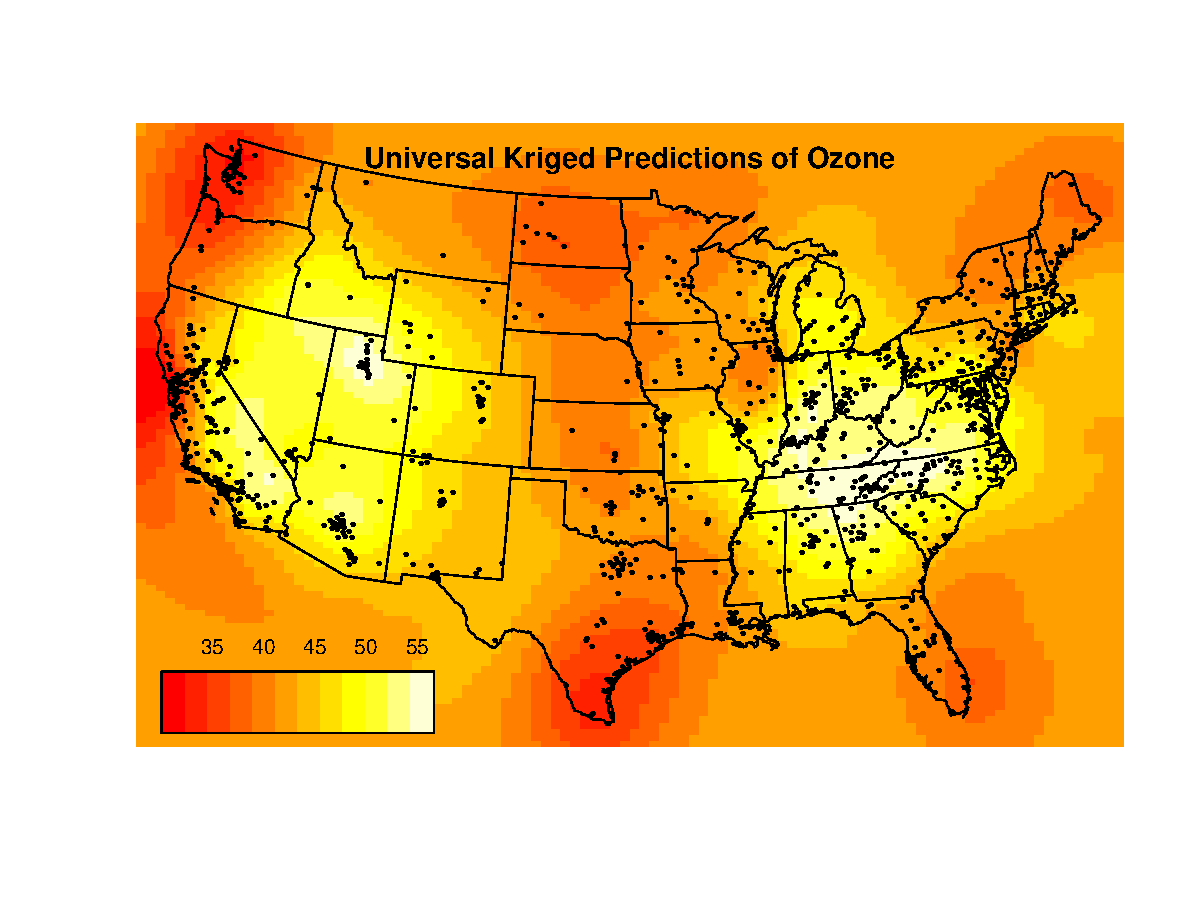
\includegraphics[width=\maxwidth]{figure/uk} 

\end{knitrout}


\begin{knitrout}
\definecolor{shadecolor}{rgb}{0.969, 0.969, 0.969}\color{fgcolor}
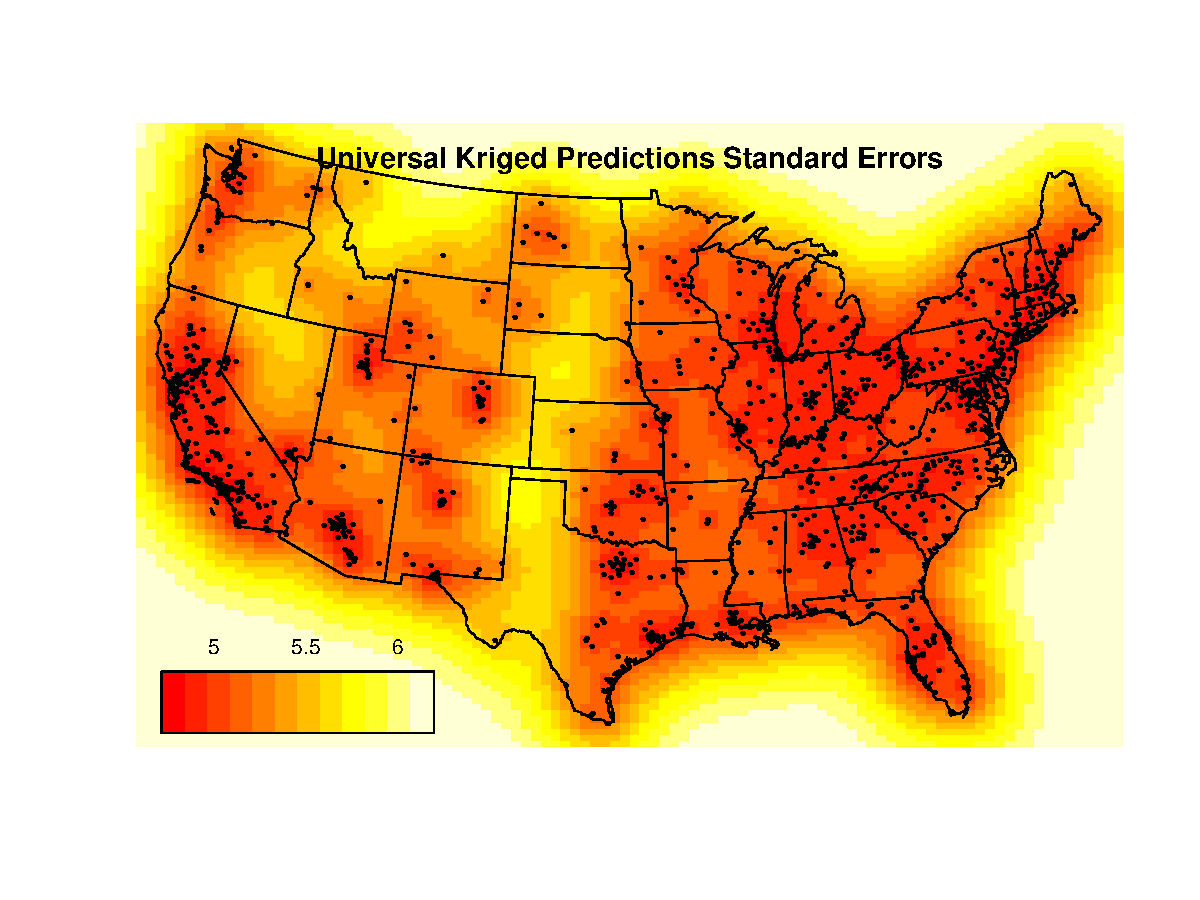
\includegraphics[width=\maxwidth]{figure/ukresid} 

\end{knitrout}


\item[l.]
With the information generated (g) - (k) address the following and reference specific plots in your answers/interpretations.
\begin{enumerate}[(i)]
\item
Write out the statistical regression models used for generating the predictions in (h) through (k). If a statistical model doesn’t exist just say so. Level of detail for the written models should be commensurate with that found in the lecture notes.

{\sf
(h) Inverse distance weighting (IDW) is not a statistical model. 

(i) The trend surface (TS) model is 
\[
Y(s) = b_0 + b_1 X(s) + \epsilon(s)
\]
where $Y(s)$ is the value of the ozone at spatial location $s$. The covariate $X(s)$ is the value of the natural spline (applied to Ozone vs Easting coordinate data) with four knots evaluated at spatial location $s$. The error terms are assumed independence with common variance, $\epsilon(s) \sim N(0, \sigma^2)$.

(j) The ordinary kriging (OK) model is
\[
Y(s) = b_0 + \epsilon(s)
\]
where $Y(s)$ is the value of the ozone at spatial location $s$. The error term is distributed as $N(0, \Sigma)$ so that $\Sigma$ can encapsulate spatial dependence. The variance matrix $\Sigma$ is approximated using a variogram that is estimated from the data $Y(s)$ with a spherical model and weighted least squares fitting.

(k) The universal kriging model is a combination of OK and TS
\[
Y(s) = b_0 + b_1 X(s) + \epsilon(s)
\]
where $Y(s)$ is the value of the ozone at spatial location $s$. The covariate $X(s)$ is the value of the natural spline (applied to Ozone vs Easting coordinate data) with four knots evaluated at spatial location $s$. The variance matrix $\Sigma$ is approximated using a variogram that is estimated from the residuals after regressing $Y$ onto $X$ with a spherical model and weighted least squares fitting.
}
\item
For each of the spatial prediction approaches considered (IDW, trend surface, ordinary and universal kriging) describe the behavior of the predictions and prediction standard errors as prediction locations get further away from the sampled data.

{\sf
IDW behaves very mechanically. It shows hot spots (higher predictions) where the original data do. It has no standard errors. Getting farther away from data points, IDW gets very smooth.

TS looks clunky because it has vertical bands. The predicted value depends only on the easting coordinate. Its standard errors are lower than the others because it assumes the errors are independent. Getting away from sampled data doesn't affect the predictions because it is only a function of the easting coordinate. The standard errors behave the same way since they are also only a function of the easting coordinate.

OK doesn't assume a large scale trend. Getting away from data points, OK predicts closer to the national average. That is a property of the model. The standard errors also grow.

For UK, as the estimated point is farther and farther away from data points, it approaches its expected value given the covariates. The standard errors are less than in OK because the including the covariate increases the $R^2$ value of the model.
}
\item
Spend some time studying the difference between the spatial prediction approaches presented with this data. There is nothing to write down or hand in for this, but I'm hoping it might generate some questions.

\textsf{Done}
\end{enumerate}
\end{enumerate}

\end{document}
